\documentclass[11pt, oneside]{article}   	% use "amsart" instead of "article" for AMSLaTeX format


% \usepackage{draftwatermark}
% \SetWatermarkText{Draft}
% \SetWatermarkScale{5}
% \SetWatermarkLightness {0.9} 
% \SetWatermarkColor[rgb]{0.7,0,0}

%
%	TikZ
%
\usepackage{tikz}
\usetikzlibrary{calc,patterns,angles,quotes,shapes,math,decorations,through,intersections,lindenmayersystems,backgrounds}    
\usepackage{tkz-euclide}
\usepackage{pgfplots}
%
%
%
\usepackage{geometry}                		% See geometry.pdf to learn the layout options
\geometry{letterpaper}                   		% ... or a4paper or a5paper or ... 
%\geometry{landscape}                		% Activate for for rotated page geometry
%\usepackage[parfill]{parskip}    		% Activate to begin paragraphs with an empty line rather than an indent
\usepackage{graphicx}				% Use pdf, png, jpg, or eps� with pdflatex; use eps in DVI mode
								% TeX will automatically convert eps --> pdf in pdflat						
								% TeX will automatically convert eps --> pdf in pdflatex		
\usepackage{amssymb}
\usepackage{mathrsfs}
\usepackage{hyperref}
\usepackage{url}
\usepackage{subcaption}
\usepackage{authblk}
\usepackage{amsmath}
\usepackage{mathtools}
\usepackage{graphicx}
\usepackage[export]{adjustbox}
\usepackage{hyperref}
\usepackage{alltt}
\usepackage{color}
\usepackage[utf8]{inputenc}
\usepackage[english]{babel}
\usepackage{float}
\usepackage{bigints}
\usepackage{braket}
\usepackage{siunitx}
\usepackage{relsize}


%
% compatability
%
\pgfplotsset{compat=1.17} 

\newcommand*{\Scale}[2][4]{\scalebox{#1}{$#2$}}%


\begin{document}



\begin{figure}[H]
  \centering
  \resizebox{0.45 \textwidth}{!} {																% resize figure if you want
    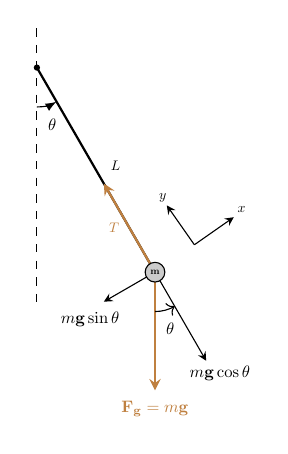
\begin{tikzpicture}
      \pgfmathsetmacro{\Gvec}{1.5}																% save length of g-vector and theta to macros
      \pgfmathsetmacro{\myAngle}{30}
      \pgfmathsetmacro{\Gcos}{\Gvec*cos(\myAngle)}												% calculate lengths of vector components
      \pgfmathsetmacro{\Gsin}{\Gvec*sin(\myAngle)}
%
%	make some coordinates
%
      \coordinate (centro) at (0,0);
      \draw[dashed] (0,0.5) -- ++(0,-3.5) node (mary) [black,below]{};
      \fill (centro) circle (0.04);
      \draw[thick] (centro) -- ++(270+\myAngle:3) coordinate (bob);
      \path (1.00,-1.25) node[] {$\Scale[0.5] {L}$}; 
      \draw [thick,brown,-stealth] (bob) -- ($(bob)!\Gcos cm!(centro)$) node[left,midway] {${\Scale[0.50] T}$};
%
%	draw the angle
%
     \pic [draw, -latex, "${\Scale[0.60]{\theta}}$", angle eccentricity=1.5] {angle = mary--centro--bob};
%
%	draw the rest of the pendulum
%
     \draw [-stealth] (bob) -- ($(bob)!-\Gcos cm!(centro)$)
       coordinate (gcos)
      node[midway,below, yshift=-0.5cm, xshift=0.50cm] {$\Scale[0.60] {m {\bf g} \cos\theta}$};
     \draw [-stealth] (bob) -- ($(bob)!\Gsin cm!90:(centro)$)
       coordinate (gsin)
     node[midway,below,yshift=-0.20cm, xshift=-0.50cm] {$\Scale[0.60] {m {\bf g} \sin \theta}$};
     \draw [thick,brown,-stealth] (bob) -- ++(0,-\Gvec)
       coordinate (g)
       node[below,brown] {$\Scale [0.60] {{\bf F_{g}} = m {\bf g}}$};
     \pic [draw, ->, "{$\Scale[0.60] {\theta}$}", angle eccentricity=1.5] {angle = g--bob--gcos};
     \filldraw [fill=black!20,draw=black] (bob) circle[radius=0.125];
     \path (bob) node[] {$\Scale[0.35] {\bf m}$};
%
%	draw the x-y coordinate system
%
     \draw [-stealth] (2.00,-2.25) -- (2.50,-1.90) node[xshift=0.10cm, yshift=0.10cm] {$\Scale[0.50] {x}$};
     \draw [-stealth] (2.00,-2.25) -- (1.65,-1.75) node[xshift=-0.05cm,yshift=0.10cm] {$\Scale[0.50] {y}$};
   \end{tikzpicture}
  }																							% end \resizebox
\caption{Free Body Diagram of a Simple Pendulum}
\label{fig:simple_pendulum}
\end{figure}


\newpage


\begin{figure}[H]
\centering
  \resizebox{0.70 \textwidth}{!} {																% resize figure if you want
  
  
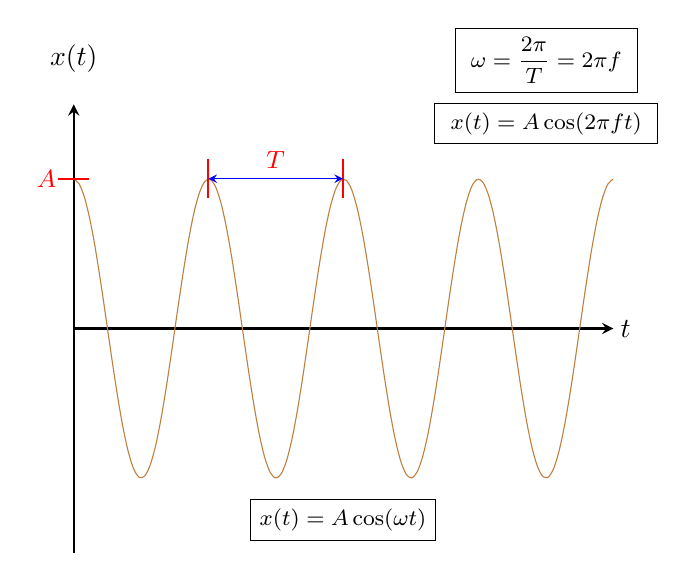
\begin{tikzpicture}
  \def \A {1.0}																					% x(t) = A cos (wt)
  \def \w {1.0}																					% x(t) = A cos (wt)
  \begin{axis}[
    axis line style = thick,
    ticks=none,
    ymin=-1.5,
    ymax=1.5,
    axis x line=middle,
    axis y line=middle,
    xlabel=$t$,
    ylabel={$x(t)$},
    every axis x label/.style={
      at={(ticklabel* cs:1.05)},
      anchor=east,
    },
    every axis y label/.style={
      at={(ticklabel* cs:1.05)},
      anchor=south,
    },
  ]
  \addplot[domain=0:(4*2*pi),samples=100,smooth,brown]{\A*cos(\w*deg(x))};
 \end{axis}
 
%
%
% \fill [red] (0.0,4.75) circle (0.05);															% draw a dot at (0,1) (not really sure how to compute this)
  \path (0.0,4.75) node[font=\small,xshift=-1.0mm,left,red] {${A}$};							% label with A
  \draw[thick,red] (-0.20,4.75) -- (0.20,4.75);													% draw a short line
  
% \fill [red] (1.71,4.75) circle (0.05);														% again, not really sure how to compute these (eyeballed)
% \fill [red]  ({2*1.71},4.75) circle (0.05);
  \draw[thick,red] (1.71,4.50) -- (1.71,5.00); 
  \draw[thick,red] ({2*1.71},4.50) -- ({2*1.71},5.00); 
  \draw[blue,stealth-stealth] (1.71,4.75) -- ({2*1.71},4.75) coordinate [label={[font=\small,midway] {${\color{red}{T}}$}}];
  \path (6.00,6.25) node[font=\footnotesize,draw,rectangle] {$\; \omega = \dfrac{2 \pi}{T} = 2 \pi f \;$}; 
  \path (6.00,5.45) node[font=\footnotesize,draw,rectangle] {$\; x(t) = A \cos (2 \pi f t) \;$}; 
  \draw[draw=none] (0.00,0.15) -- ({4*1.71},0.15) coordinate [label={[draw,rectangle,font=\footnotesize,midway] {$x(t) = A \cos (\omega t)$}}];
 \end{tikzpicture}
}
\caption{SMH Displacement Function}
\label{fig:smh_displacement_function}
\end{figure}




\begin{figure}[H]
\centering
  \resizebox{0.90 \textwidth}{!} {															% resize figure if you want
   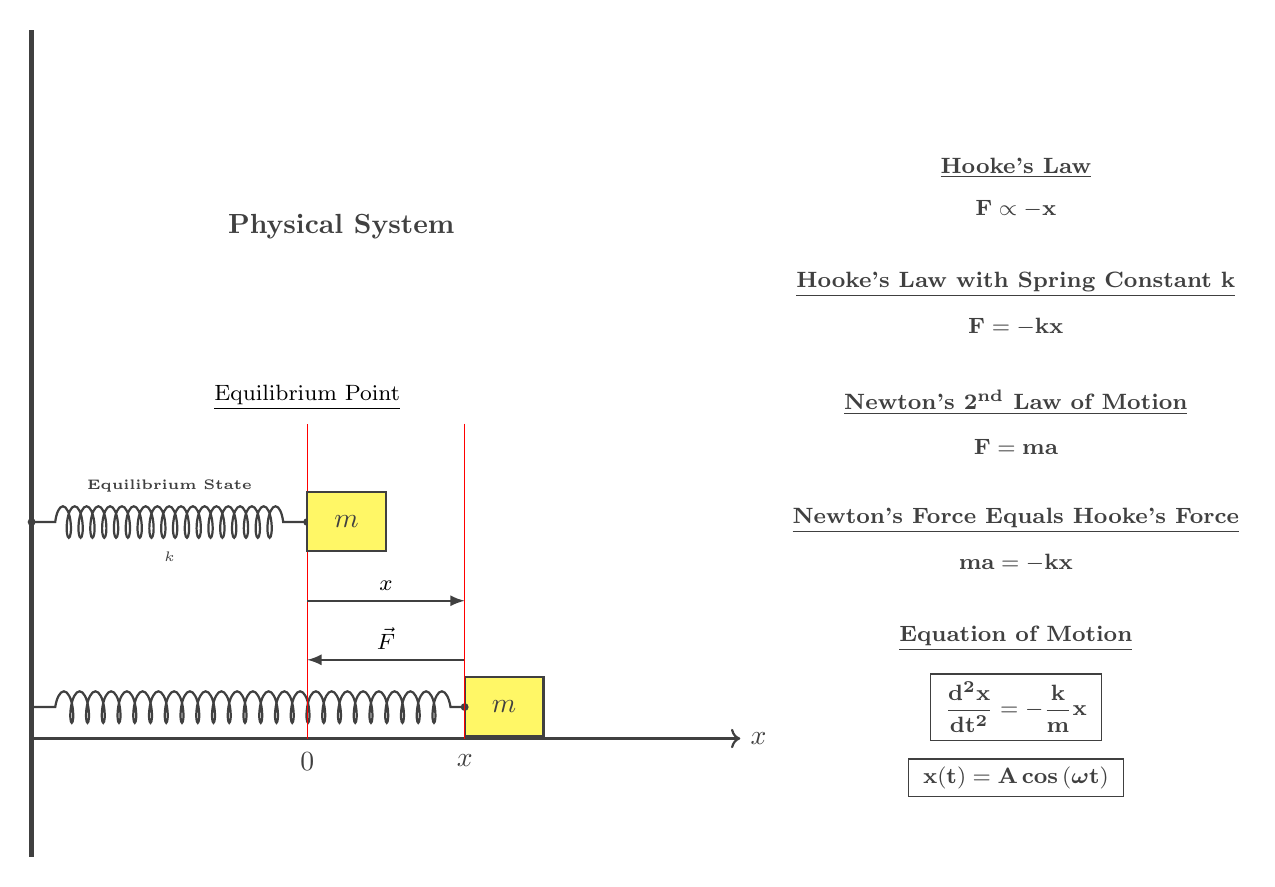
\begin{tikzpicture}[black!75,thick]														% draw the picture
        \draw[thick, ->] (0.00,0.00) -- (9.00,0.00) coordinate [label={[right] $x$}];		% draw x axis     
        \draw[ultra thick] (0.00,-1.50) -- (0.00,9.00);										% this is the support (y axis, I guess)

%
% draw the first spring 
%
        \draw [
              decoration={
                 coil,
                 aspect=0.3, 
                 segment length=2mm, 
                 amplitude=2mm, 
                 pre length=3mm,
                 post length=3mm},
             decorate] (0,0.40) -- (5.75,0.40);
ç %      \draw[draw=none] (0,0.15) -- (1.75,0.15) coordinate [label={[yshift=0.5cm] k}];		% draw k
 %      
 %
 %
 % draw the first mass
 %
       \node[draw,
	     fill=yellow!60,
	     minimum width=1cm,
	     minimum height=0.75cm,
	     anchor=north,
	     label=center:$m$] at (6,0.80) {};
	     
      \fill (5.5,0.40) circle(0.05);   
      \path (5.5,0.0) node[yshift=-0.75mm, below] {$x$}; 
%
%	make some coordinates
%        
      \coordinate (c1) at (5.50,6.50);
      \coordinate (c2) at (3.50,0.00);
      \coordinate (c3) at (3.50,4.00);            
 %
 %	draw some text
 %  
      \path (c1) node[left] {\bf Physical System};
      \path (c2) node[yshift=-0.5mm, below] {$0$};
      \draw[thin,red] (c2) -- (c3) coordinate [label={[above, yshift=0.5mm] \text{{\footnotesize \color{black}{{\underline{Equilibrium Point}}}}}}];   
      \draw[-latex]   (3.50,1.75) -- (5.50,1.75) coordinate [label={[font=\footnotesize,color=black,midway,above] {$x$}}];
      \draw[latex-]   (3.50,1.00) -- (5.50,1.00) coordinate [label={[font=\footnotesize,color=black,midway,above] {$\vec{F}$}}]; 
      \draw[thin,red] (5.50,4.00) -- (5.50,0.00);
%
% draw the second spring 
%
        \draw [
              decoration={
                 coil,
                 aspect=0.3, 
                 segment length=1.5mm, 
                 amplitude=2mm, 
                 pre length=3mm,
                 post length=3mm},
             decorate] (0.00,2.75) -- (3.5,2.75);
        \draw [draw=none] (0.00,2.75) -- (3.50,2.75) coordinate [label={[midway,above,yshift=0.25cm] \text{{\tiny {\bf Equilibrium State}}}}];  
        \fill (0.00,2.75) circle(0.05);																				% draw a dot connecting the spring to the y axis
        \fill (3.50,2.75) circle(0.05);																				% draw a dot connecting the spring to the mass
        \draw [draw=none] (0,2.75) -- (3.5,2.75) coordinate [label={[midway,below,yshift=-0.25cm] {\tiny $k$}}];	% draw k

 %
 % draw the second mass
 %
       \node[draw,
	     fill=yellow!60,
	     minimum width=1cm,
	     minimum height=0.75cm,
	     anchor=north,
	     label=center:$m$] at (4.00, 3.15) {};
	     
%	
%	draw information about the graphic to the right ((12.00,Y))
%
%	mostly eyeballed
%

	     \begin{footnotesize}
	       \draw [draw=none] (12.00,7.00) -- (13.00,7.00) coordinate [label={[midway] \underline{{\bf Hooke's Law}}}]; 
	   	   \draw [draw=none] (12.00,6.50) -- (13.00,6.50) coordinate [label={[midway] {${\mathbf {\displaystyle F \propto -x}}$}}];
		   \draw [draw=none] (12.00,5.50) -- (13.00,5.50) coordinate [label={[midway] \underline{{\bf Hooke's Law with Spring Constant $\mathbf {k}$}}}]; 
		   \draw [draw=none] (12.00,5.00) -- (13.00,5.00) coordinate [label={[midway] {${\mathbf {\displaystyle F = -kx}}$}}];
		   \draw [draw=none] (12.00,4.00) -- (13.00,4.00) coordinate [label={[midway] \underline{{\bf Newton's ${\mathbf 2^{\text{nd}}}$ Law of Motion}}}]; 
		   \draw [draw=none] (12.00,3.50) -- (13.00,3.50) coordinate [label={[midway] {${\mathbf {\displaystyle F = ma}}$}}];
		   \draw [draw=none] (12.00,2.50) -- (13.00,2.50) coordinate [label={[midway] \underline{{\bf Newton's Force Equals Hooke's Force}}}];
		   \draw [draw=none] (12.00,2.00) -- (13.00,2.00) coordinate [label={[midway] {${\mathbf {\displaystyle ma = -kx}}$}}];
		   \draw [draw=none] (12.00,1.00) -- (13.00,1.00) coordinate [label={[midway] \underline{{\bf Equation of Motion}}}]; 
		   \draw [draw=none] (12.00,0.40) -- (13.00,0.40) node[thin,draw,rectangle,midway] 
		   					 {${\; \mathbf {\dfrac{d^2 x}{dt^2} = -\dfrac{k}{m} x\;}}$};			 
		   \draw [draw=none] (12.00,-0.50) -- (13.00,-0.50) node[thin,draw,rectangle,midway] 
		   					 {${\; \mathbf {x(t) = A \,{\boldsymbol\cos} \, ({\boldsymbol \omega} t)\;}}$};
		 \end{footnotesize}
		 
    \end{tikzpicture}
  }																				% end resizebox                                                                                           
\caption{Spring and Mass System with Spring Constant $k$ and Mass $m$}
\label{fig:spring_and_mass_system}
\end{figure}

\bigskip

%
%	draw Pythagorean theorem stuff
%
\begin{figure}[H]
\centering
  \resizebox{0.75 \textwidth}{!} {																							% resize figure if you want
  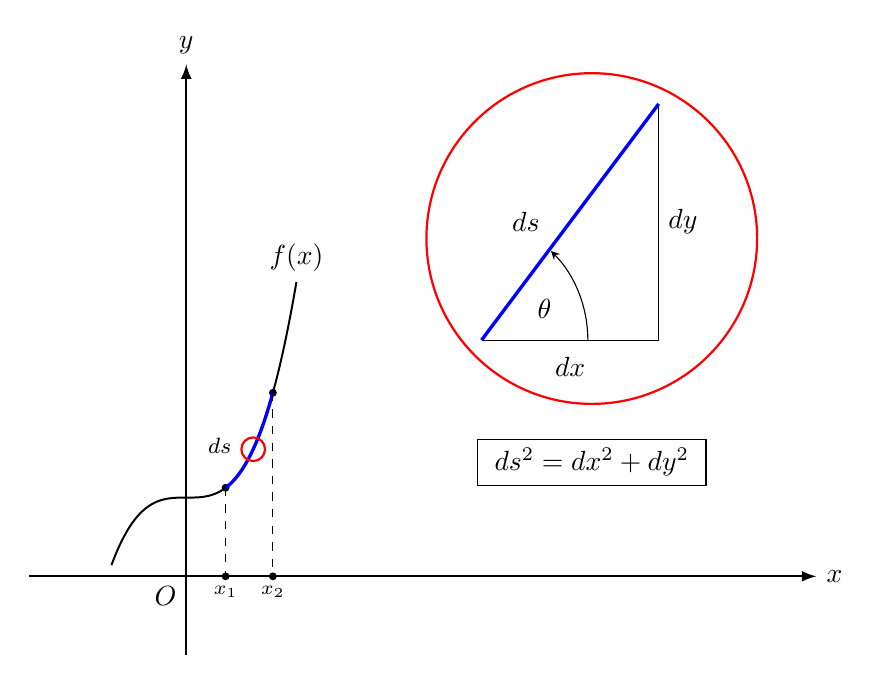
\begin{tikzpicture} [every edge quotes/.append style = {anchor=south, sloped},declare function={f(\x)=1 + \x*\x*\x;}]		% define f(x)
       \draw[thick, -latex] (-2,0) -- (8.0,0.0) coordinate [label={[right] $x$}];  											% x axis
       \draw[thick, -latex] (0,-1) -- (0,6.5) coordinate [label={[above] $y$}]; 											% y axis
       \draw [line width=0.25mm, smooth,samples=100,domain=-0.95:1.40] plot (\x,{f(\x)});									% draw f(x)
       \draw [draw=none] (1.40, {f(1.40)}) coordinate [label={[above] $f(x)$}];												% label f(x)
       \coordinate (O) at (0,0); 																							% origin
       \path (O) node[below left] {$O$};																					% draw origin
%
%	various coordinates
%     
       \coordinate (x1y1) at (0.5,{f(0.5)});
       \coordinate (x1y0) at (0.5,0.0);
       \coordinate (x2y2) at (1.1,{f(1.1});
       \coordinate (x2y0) at (1.1,0.0);
       \coordinate (cir)  at (0.85,{f(0.85)});
%
       \fill (x1y1) circle (0.05);																					% put a dot on the curve at x1y1
       \fill (x2y2) circle (0.05);																					% put a dot on the curve at x2y2
	   \draw [very thick,blue,smooth,samples=100,domain=0.5:1.1] plot (\x,{f(\x)});									% draw blue segment on f(x)
       \draw[draw=none] (x1y1) -- (x2y2) coordinate [label={[font=\footnotesize,yshift=-0.065cm,xshift=-0.105cm,midway,left] \color{black} $ds$}];
       \draw[dashed] (x1y1) -- (x1y0) coordinate [label={[font=\scriptsize,below] \color{black} $x_1$}];
       \draw[dashed] (x2y2) -- (x2y0) coordinate [label={[font=\scriptsize,below] \color{black} $x_2$}];
       \fill (x1y0) circle (0.05);																					% put a dot on the x axis at x1
       \fill (x2y0) circle (0.05);																					% put a dot on the x axis at x2
       \draw[red, thick] (cir) circle (0.150);																		% put a circle on f(x) where ds is
       

     
%
%	draw triangle and circle to show ds
%   
%
%
%	set up triangle coordinates
%
	   \coordinate (a) at (3.75,3.00);
	   \coordinate (c) at (6.00,3.00);
	   \coordinate (b) at (6.00,6.00);
%
%	draw the triangle
%	   
       \draw[] (a) -- (c) coordinate [label={[yshift=-0.1cm,midway,below] ${dx}$}];										% dx
       \draw[] (c) -- (b) coordinate [label={[midway,right] ${dy}$}];													% dy
       \draw[blue,very thick] (a) -- (b) coordinate [label={[xshift=-0.25cm,midway,left] \color{black} ${ds}$}];		% ds
       \draw[red,thick] (5.15,4.29) circle (2.10);																		% big circle
       \draw[draw=none] (0,0) -- (5.15,1.75)  node[draw,rectangle,below] {${\; ds^2 = dx^2 + dy^2 \;}$};				% draw the pythagorean theorem
%
%	draw the angle      
%       
       \node[xshift=-2mm, yshift=-2mm] at (4.75,3.60) {$\theta$};
       \draw[-stealth,thin] (5.10,3.00) arc (0:45:1.60cm);
%
%	done
%
     \end{tikzpicture}
    }																					 								% end resizebox                                                            
 \caption{$f(x)$, $ds$ and the Pythagorean Theorem}
 \label{fig:pythagorean_theorem}
\end{figure}



\begin{figure}[H]
  \centering
  \resizebox{0.30 \textwidth}{!} {											% resize the figure if you want
    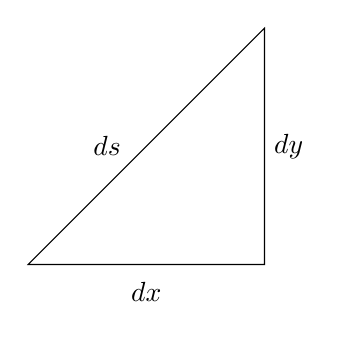
\begin{tikzpicture}
      \draw (0,0) coordinate[] (a) --
            (3,0) coordinate[] (c) --
            (3,3) coordinate[] (b) -- cycle;
       \draw[draw=none] (a) -- (c) coordinate [label={[yshift=-0.1cm,midway,below]	${dx}$}];    % dx
       \draw[draw=none] (c) -- (b) coordinate [label={[midway,right]  				${dy}$}];    % dy
       \draw[draw=none] (a) -- (b) coordinate [label={[xshift=-0.2cm,midway,left]	${ds}$}];    % ds
    \end{tikzpicture}
  }
 \caption{$ds^2 = dx^2 + dy^2$}
 \label{fig:ds}
\end{figure}



\begin{figure}[H]
  \centering
  \resizebox{0.75 \textwidth}{!} {											% resize the figure if you want
    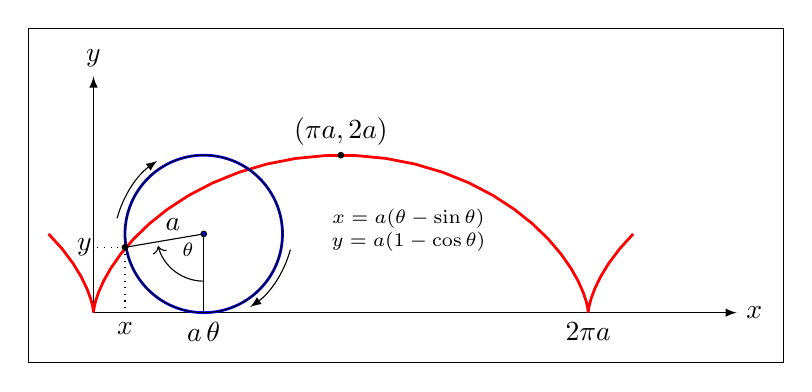
\begin{tikzpicture} [framed]											% draw the picture inside a black frame (requires \usetikzlibrary{backgrounds})
     \coordinate (O) at (0,0);
     \coordinate (A) at (0,3);
     \def\r{1}                                                          	% r is the radius
     \def\c{1.4}                                                        	% c is the center
     \coordinate (C) at (\c, \r);

     \draw[-latex] (O) -- (A) node[anchor=south] {$y$};
     \draw[-latex] (O) -- (2.6*pi,0) node[anchor=west] {$x$};
     \draw[red,domain=-0.5*pi:2.5*pi,samples=50, line width=1] plot ({\x - sin(\x r)},{1 - cos(\x r)});
     \draw[blue, line width=1] (C) circle (\r);
     \draw[] (C) circle (\r);
%
%       set up some variables and coordinates
%
     \def\x{0.4}                                                        	% x
     \def\y{0.83}															% y
     \def\xa{0.3} 															% coordinate x for arc left
     \def\ya{1.2} 															% coordinate y for arc left
     \coordinate (X) at (\x, 0 );
     \coordinate (Y) at (0, \y );
     \coordinate (XY) at (\x, \y );
     \node[anchor=north] at (X) {$x$} ;

     \draw[fill=blue] (C) circle (1pt);   									% draw center of circle
     \draw[] (C) -- node[anchor=south] {\; $a$} (XY);   					% draw radius of the circle
     \coordinate (B) at (\c, 0);    										% bottom of circle, radius to the bottom
     \draw[] (C) -- (B) node[anchor=north] {$a \, \theta$};
%
%       projections of point XY
%
     \draw[dotted] (XY) -- (X);
     \draw[dotted] (XY) -- (Y) node[anchor=east, xshift=1mm] {$\quad y$};
%
%       arc theta
%       start arc
%
     \coordinate (S) at (\c, 0.4);
     \draw[->] (S) arc (-90:-165:0.6);
     \node[xshift=-2mm, yshift=-2mm] at (C) {\scriptsize $\theta$};
%
%       arc above
%
     \coordinate (AA) at (\xa, \ya);
     \draw[-latex, rotate=25] (AA) arc (-220:-260:1.3);
%
%       arc below
%
     \def\xb{2.5}                                                               % coordinate x for arc bottom
     \def\yb{0.8}                                                               % coordinate y for arc bottom
     \coordinate (AB) at (\xb, \yb);
     \draw[-latex, rotate=-10] (AB) arc (-5:-45:1.3);
     \draw[fill=black] (XY) circle (1pt);                                        % draw XY dot
%
%       top label
%
     \coordinate (T) at (pi, 2);
     \node[anchor=south] at (T)  {$(\pi a, 2 a )$} ;
     \draw[fill=black] (T) circle (1pt);
%
%       equations
%
     \coordinate (E) at ( 4,1.2);
     \coordinate (F) at ( 4,0.9);
     \node[] at (E) {\scriptsize $x=a(\theta - \sin \theta)$};
     \node[] at (F) {\scriptsize $y=a(1 - \cos \theta)$};
%
%       label 2pi a
%
     \coordinate (TPA) at (2*pi, 0);
     \node[anchor=north] at (TPA) {$2 \pi a$};
    \end{tikzpicture}
  }
 \caption{The Cycloid Curve}
 \label{fig:cycloid}
\end{figure}


%
%	brachistochrone problem setup
%
\begin{figure}[H]
  \centering
  \resizebox{0.65 \textwidth}{!} {										% resize the figure if you want
     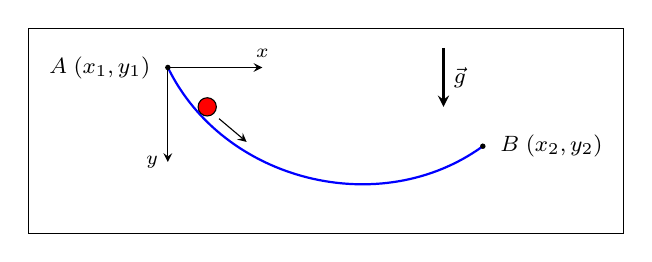
\begin{tikzpicture} [framed]										% draw the picture inside a black frame (requires \usetikzlibrary{backgrounds})
%
%	set up some coordinates
%
        \coordinate (A)		at (0.0,  0.0);								% put the origin at A
        \coordinate (Ax)	at (1.2,  0.0);								% x axis here
        \coordinate (Ay)	at (0.0, -1.2);								% y axis positive in the down direction
        \coordinate (Ball)	at (0.5, -0.5);								% draw the ball here
        \coordinate (B)		at (4.0, -1.0);								% other end of the curve
        \coordinate (Gy0)	at (3.5,  0.25);							% draw the gravity vector starting here
        \coordinate (Gy1)	at (3.5, -0.5);								% gravity vector ends here
        \coordinate (D0)	at (0.65,-0.65);							% draw motion arrow starting here
        \coordinate (D1)	at (1.0, -0.945);							% motion arrow ends here
%
%	draw the picture
%
        \draw[blue, thick] (A) to [bend right=50] (B);					% draw the curve in blue
        \node[circle, draw=black, fill=red, scale=0.70] at (Ball) {};	% draw a red ball with a black outline on the curve
        \draw[-stealth, thin] (D0) -- (D1);								% draw an arrow in the direction the ball is moving
        \fill (A) circle (0.035);										% put a dot on the curve at A
        \fill (B) circle (0.035);										% put a dot on the curve at B
        \draw[draw=none] (A) node[xshift=-0.10cm, font=\footnotesize, left] {$A \; (x_1,y_1)$};						% label A
        \draw[draw=none] (B) node[xshift=0.10cm, font=\footnotesize, right] {$B \; (x_2,y_2)$};						% label B
        \draw[-stealth, thin] (A) -- (Ax) coordinate [label={[font=\scriptsize, above] $x$}];						% draw x axis
        \draw[-stealth, thin] (A) -- (Ay) coordinate [label={[font=\scriptsize, left] $y$}];						% draw y axis
        \draw[-stealth, thick] (Gy0) -- (Gy1) coordinate [label={[font=\footnotesize, midway, right] $\vec{g}$}];	% draw the gravity vector (g)
      \end{tikzpicture}													% end \tikzipcture
    }																	% end \resizebox
  \caption{The Brachistochrone Problem Setup}
  \label{fig:brachistochrone}
\end{figure}




\def\level{5}
\begin{figure}[H]
  \centering
  \resizebox{0.45 \textwidth}{!} {                                                                                                                                                            % resize figure if you want
      \begin{tikzpicture}[l-system={step=5pt, order=\level, angle=120},rotate=180]
         \pgfdeclarelindenmayersystem{Sierpinski triangle}{
         \symbol{X}{\pgflsystemdrawforward}
         \symbol{Y}{\pgflsystemdrawforward}
          \rule{X -> X-Y+X+Y-X}
          \rule{Y -> YY}
        }
        \draw [black] (3,2) l-system [l-system={Sierpinski triangle, axiom=X, anchor=north east},fill=white];
      \end{tikzpicture}
    }
  \caption{Sierpiński triangle/gasket}
  \label{fig:sierpinski}
\end{figure}





\begin{figure}[H]
\centering
  \resizebox{0.45 \textwidth}{!} {                                                                                                                                                            % resize figure if you want
   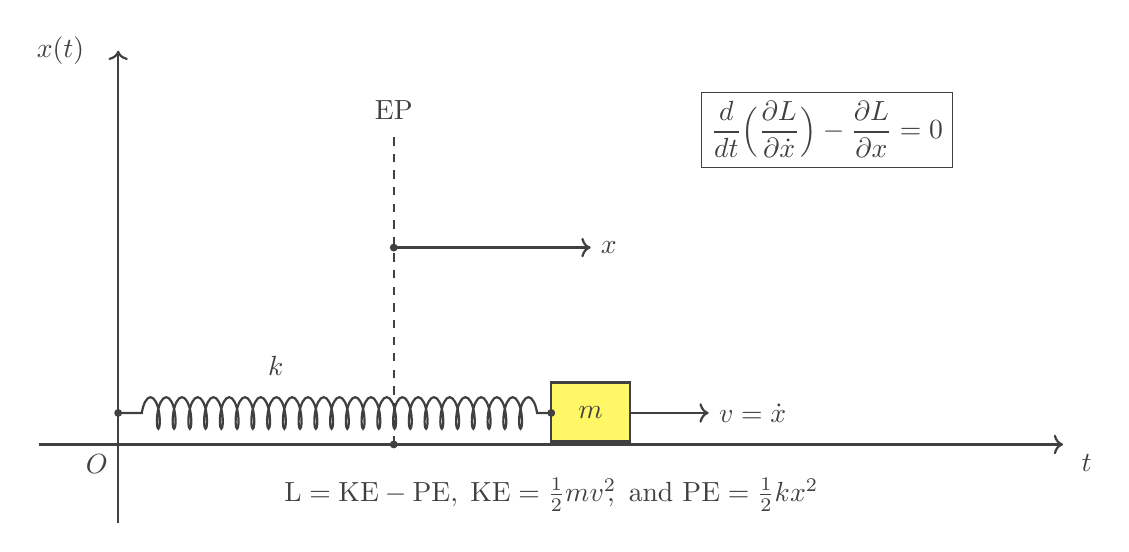
\begin{tikzpicture}[black!75,thick]
        \draw[thick, ->] (-1,0) -- (12,0) coordinate [label={[xshift=0.30cm, below] $t$}];                                                                          % horizontal axis
        \draw[thick, ->] (0,-1) -- (0,5) coordinate [label={[xshift=-0.30cm, left] $x(t)$}];                                                                           % xshift -- get some extra space
        \draw[draw=none] (-1,0) -- (12,0) coordinate [label={[yshift=-0.3cm,midway,below] 
                                      ${\text{L} = \text{KE} - \text{PE}, \; \text{KE} = \frac{1}{2} m v^2 \!\!, \text{ and PE} = \frac{1}{2} k x^2}$}];    % draw the equations below the x axis
        \draw (9,4) node[rectangle, draw, very thin] 
                         {$\mathlarger {\dfrac{d}{dt} \Big ( \dfrac{\partial L}{\partial \dot{x}} \Big ) - \dfrac{\partial L}{\partial x} = 0}$};             % draw the Euler-Lagrange equation to the right
       \path (0,0) node[below left] {$O$};    

%
% draw the spring 
%
        \draw [
              decoration={
                 coil,
                 aspect=0.3, 
                 segment length=2mm, 
                 amplitude=2mm, 
                 pre length=3mm,
                 post length=3mm},
             decorate] (0,0.40) -- (5.75,0.40);
        \fill (0,0.40) circle(0.05);                                                                                                                                                                 % draw a dot connecting the spring to the y axis

 %
 % draw the mass
 %
       \node[draw,
	     fill=yellow!60,
	     minimum width=1cm,
	     minimum height=0.75cm,
	     anchor=north,
	     label=center:$m$] at (6,0.80) {};
      \fill (5.5,0.40) circle(0.05);                                                                                                                                                                 % draw a dot connecting the mass to the spring

       
      \draw[->] (6.5,0.40)-- (7.5,0.40) coordinate [label={[right] ${v = \dot{x}}$}];                                                                                              % draw velocity vector (v) to the right of the mass
      
%
% other annotation of axes etc
%
      \coordinate (k) at (2,1.25);
      \draw[draw=none] (k) node[below] {$k$};    
      \coordinate (c1) at (3.5,0);
      \coordinate (c2) at (3.5,4);
      \coordinate (c3) at (3.5,2.5);
      \coordinate (c4) at (6,2.5);
      \draw[dashed] (c1) -- (c2) coordinate [label={[above] EP}];   
      \draw[->] (c3) -- (c4) coordinate [label={[right] $x$}];   
      \fill (c1) circle(0.05);      
      \fill (c3) circle(0.05);      
    \end{tikzpicture}
  }                                                                                                                                                                                                                     % end resizebox                                                                                           
\caption{Simple Harmonic Motion Setup}
\label{fig:shm}
\end{figure}


\begin{figure}[H]
\centering
  \resizebox{0.65 \textwidth}{!} {                                                                                                                                                % resize figure if you want
  \begin{tikzpicture} [every edge quotes/.append style = {anchor=south, sloped}, declare function={f(\x)=\x*\x + 1;}]             % define f(x)
       \draw[thick, ->] (-5,0) -- (5,0) coordinate [label={[xshift=0.30cm, below] $x$}];                                                                 % horizontal axis
       \draw[thick, ->] (0,-1) -- (0,5) coordinate [label={[xshift=-0.30cm, left] $f(x)$}];                                                                 % xshift -- get some extra space
       \draw [line width=0.20mm, smooth,samples=100,domain=-1.75:1.75] plot (\x,{f(\x)});                                                                                     % draw f(x)
       \path (0,0) node[below left] {$O$};    
       \coordinate (p) at (0,{f(0)});                                                                                                                                                % draw a dot at minimum
       \coordinate (x) at (0,{1/(4*f(1))});                                                                                                                                        % coordinate for tangent line
       \node[very thick, circle through={(p)}] (cir) at (x) {};
       \draw[line width=0.25mm,red] (-3,{f(0)})-- (3,{f(0)});
       \fill (p)circle (0.05);                                                                                                                                                             % draw a dot at minimum (draw last to ensure it's black)
%
% draw dots on curve and axis
%
       \coordinate (e0) at (0.15,0);
       \fill (e0) circle(0.05);      
       \coordinate (e1) at (0.15,{f(0)});
       \fill (e1) circle(0.05);      
       \draw[dashed] (0.15,{f(0)}) -- (0.15,0) coordinate [label={[scale=1.10, below]  $\epsilon$}];                                            % draw epsilon under dot     
       \draw (5.5,1) node[rectangle, draw, very thin] {$\displaystyle \dfrac{d}{dx} f(x)  = \dfrac{d}{dx} f(x + \epsilon) = 0$};      % show derivatives at zero in box to the right
   \end{tikzpicture}
   }                                                                                                                                                                                             % end resizebox                                                                                           
 \caption{${\displaystyle f(x)= x^2 + 1}$}
 \label{fig:parabola}
\end{figure}





\begin{figure}[H]
\centering
  \resizebox{0.65  \textwidth}{!} {                                                                                                                                                 % resize figure if you want
    \begin{tikzpicture}  [every edge quotes/.append style = {anchor=south, sloped}]
       \draw[thick, ->] (-0.35,0) -- (13,0) coordinate [label={[xshift=0.30cm, below]  $t$}] (t);                                                        % xshift -- get some extra space
       \draw[thick, ->] (0,-0.35) -- (0,11) coordinate [label={[xshift=-0.30cm, left]  $x$}] (x);                                                          % xshift -- get some extra space
       \coordinate[label=below left:$ O $] (O); 
%
% draw legend
%        
       \draw (7,8) node[right,rectangle] {$x(t)$}; 
       \draw [very thick] (9.5,8) -- (11,8);
       \draw (7,7)  node [right,rectangle] {${x(t) + \eta(t)}$};
       \draw [very thick,red,dashed] (9.5,7) -- (11,7);

%
% make some coordinates for later use
%
       \coordinate (x2) at (0,5);
       \coordinate (x1) at (0,2);
       \coordinate (t2) at (6,0);
       \coordinate (t1) at (2,0);
       \coordinate (t1x1) at (2,2);
       \coordinate (t2x2) at (6,5);
         
       \draw[draw=none] (x2) node[left] {$x_2$};
       \draw [] (t2) node[below] {$t_2$};
       \draw[draw=none] (x1) node[left] {$x_1$};     
       \draw[draw=none] (t1) node[below] {$t_1$};    
%
% draw points
%
         \fill (x2) circle(0.05);      
         \fill (x1) circle(0.05);                                                                                                                                                   % draw dots on axes
         \fill (t2) circle(0.05); 
         \fill (t1) circle(0.05);  
         \fill (t1x1) circle(0.05);   
         \fill (t2x2) circle(0.05);       
         
%
% the coordinates of the parabolas are unfortunately pretty much eyeballed
%
         
        \draw[yshift=-2cm, very thick,black] (2, 4) parabola[bend={+(0, 3)}, bend pos=0.5] (6, 7);                                       % draw parabolas
        \draw[yshift=-2cm, dashed, very thick,red] (2, 4) parabola[bend={+(0, 5)}, bend pos=0.5] (6, 7);     
        \coordinate (p1) at (4,6.5);                                                                                                                                         % coordinates on curves 
        \coordinate (p2) at (4,8.5);
        \draw[dashed,thick, <->] (p1) -- (p2) coordinate [label={[midway, right]  $\eta(t)$}];                                                 % draw \eta(t) between curves                                                                              
      
 %
 % draw the S integral in a box to the right
 %        
       \draw (9.5,2.5) node[draw,thick,rectangle] {$\mathlarger {\mathlarger {{\displaystyle \mathcal{S} = \int_{t_1}^{t_2} (KE - PE) \; dt}}}$}; 
    \end{tikzpicture}
  }                                                                                                                                                                                             % end resizebox                                                                                           
 \caption{Principle of Least Action Setup}
 \label{fig:pola}
\end{figure}


%%
\begin{figure}[H]
\centering
  \begin{tikzpicture}[>=stealth, inner sep=3pt,scale=2.5]
    \draw[->] (-1.5,0) --node[below left]{$O$} (1.5,0) coordinate[label=below:$\mathbb{R}$](x);               % make and label the axes
    \draw[->] (0,-1.5) -- (0,1.5) node[left]{$\mathbb{I}$};
    \draw (0,0) coordinate(o) circle [radius=1cm];                                                                                       % draw unit circle
    \coordinate (p) at (60:1);                                                                                                                        % 60 radians with r = 1
    \fill (p) coordinate[label={above right: ${e^{i\theta} = \cos \theta + i \sin \theta}$}] (p) circle(0.02);       % Euler's formula
    \coordinate (q) at (p|-o);
%
% draw the various 1s around the unit circle
%
   \coordinate (a) at (0,1);
   \fill (a) coordinate [label={above:${1}$}] (a) circle(0.02);
   \coordinate (b) at (-1,-0);
   \fill (b) coordinate [label={left:${-1}$}] (b) circle(0.02);
   \coordinate (c) at (0,-1);
   \fill (c) coordinate [label={below:${-1}$}] (c) circle(0.02);
   \coordinate (d) at (1,0);
   \fill (d) coordinate [label={right:${1}$}] (d) circle(0.02);
%
% do the rest of the labeling
%
   \draw[thick,line join=round] (o)--node[above,left]{$r$}(p);
   \draw [dashed] (p)--(q) node [midway, right]{${\sin \theta}$};
   \draw [] (q) -- (o) node [midway, below] {${\cos x}$};
 %
 % draw the angle
 %
   \pic[draw=red,"$\theta$",angle radius=15pt,angle eccentricity=1.5,->]{angle=x--o--p};
  \end{tikzpicture}
\label{fig:eulers_formula}
\caption{Euler's Formula in the Complex Plane}
\end{figure}


\begin{figure}
\centering   
  \resizebox{0.40 \textwidth}{!} {                                                                                                                                            % resize figure if you want
\begin{tikzpicture}
  \draw[->] (-3, 0) -- (4.2, 0) node[right] {$x$};
  \draw[->] (0, -3) -- (0, 4.2) node[above] {$y$};
  \draw[scale=0.5, domain=-3:3, smooth, variable=\x, blue] plot ({\x}, {\x*\x});
  \draw[scale=0.5, domain=-3:3, smooth, variable=\y, red]  plot ({\y*\y}, {\y});
\end{tikzpicture}
}
\caption{This is a graphing test}
\end{figure}


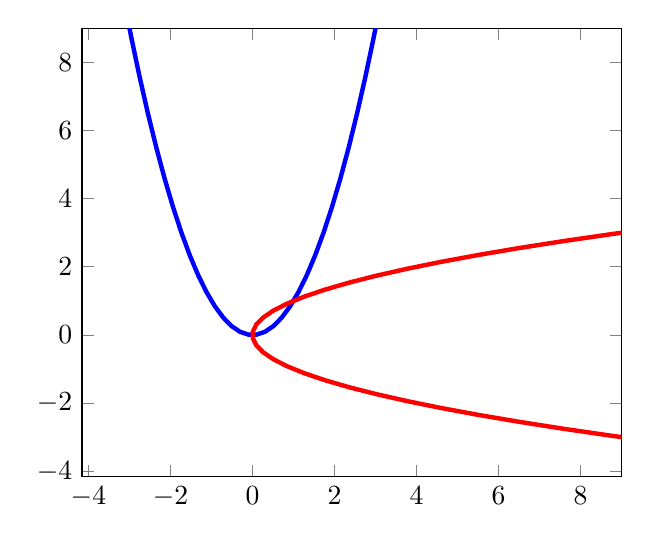
\begin{tikzpicture}
\begin{axis}[xmax=9,ymax=9, samples=50]
  \addplot[blue, ultra thick] (x,x*x);
  \addplot[red,  ultra thick] (x*x,x);
\end{axis}
\end{tikzpicture}


     \pgfplotsset{%
      every tick label/.append style = {font=\tiny},
      every axis label/.append style = {font=\scriptsize}
    }
      \resizebox{0.60 \textwidth}{!} {                                                                                                                                            % resize figure if you want

    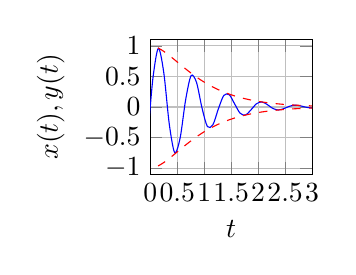
\begin{tikzpicture}
      \begin{axis}[grid=major, xmin=0, xmax=3, ymin=-1.1, ymax=1.1,
        xlabel=$t$, ylabel={$x(t), y(t)$},
        xtick = {0,0.5,...,3}, ytick = {-1,-0.5,...,1},
        scale=0.3, restrict y to domain=-1:1]
        \addplot[blue, samples=100, smooth, unbounded coords=discard]
          plot (\x, { 1 + 2 * \x)*exp(-2*\x) * sin(180* 3.14 * \x) });
        \addplot[red, dashed, samples=100, smooth]
          plot (\x, { (1+2*\x) * exp(-2*\x) } );
        \addplot[red, dashed, samples=100, smooth]
          plot (\x, { -(1+2*\x) * exp(-2*\x) } );
      \end{axis}
    \end{tikzpicture}
    }
    
\begin{tikzpicture}[scale=0.8, samples=100]
\draw[->] (-3.8,0) -- (5,0) node[right] {$x$};
\draw[->] (0,-4) -- (0,5) node[left] {$y$};
\node at (-2.8,-3)[above] {\footnotesize\color{gray} $y=x$};
\draw[smooth, domain=-3.8:2.3, color=green, thick] 
    plot (\x,{2^(\x)}) node [right] {\footnotesize $f(x)=2^x$};
\fill [green] ($(0,1)$) circle (1.5pt) node at (0,1.2)[left] {\color{green}$(0,1)$};
\draw[smooth, domain = 0.06:5, color=blue, thick] plot (\x,{log2(\x)});
\fill [blue] ($(1,0)$) circle (1.5pt) node at (1.4,0)[below] {\color{blue}$(1,0)$};
\node at (4.6,2.4)[above] {\footnotesize\color{blue}$f^{-1}(x)=\log_2 x$};
\draw[smooth, dashed, domain=-2.5:4.5, color=gray] plot (\x,\x);
\end{tikzpicture}

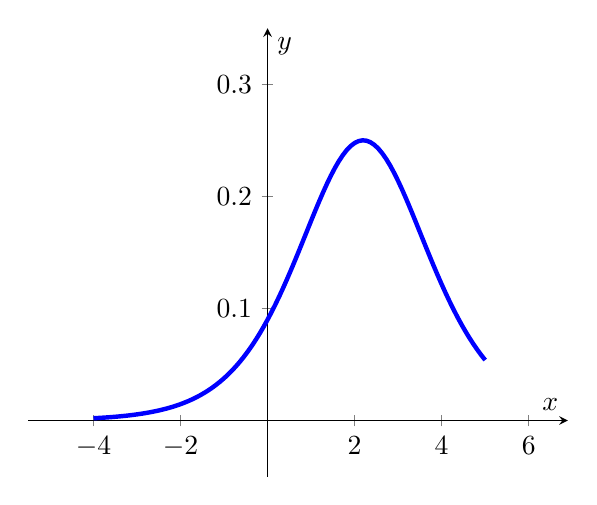
\begin{tikzpicture}
\begin{axis}[
    axis lines=middle,
    xmax=6.9,
    xmin=-5.5,
    ymin=-0.05,
    ymax=0.35,
    xlabel={$x$},
    ylabel={$y$},
    ]
    \addplot [domain=-4:5, samples=100, ultra thick, blue] {9*exp(x)/(exp(x)+9)^2};
\end{axis}
\end{tikzpicture}



\end{document}
